Here you can see how to include an image in your document.

\subsection{Product perspective}
DREAM is a functional multi-user software platform which purpose is to provide functionalities described in section \ref{sect:product_functions}. The software 

\subsubsection{User interfaces} % TODO revise te verbs
According to the assignment document the system should interact with 3 different user classes: policy makers, farmers and agronomists. In order to be more accessible and to fulfill the above mentioned professional figures needs the application should be supported by different devices. These users should interface to the service through electronic devices with an internet connection. Users that needs to access the service will have the possibility to connect throught:
\begin{itemize}
    \item an internet browser, addressing a specific web domain such as \textit{www.dream.com} that permits users to sign up/in a dedicated web application;
    \item a mobile application that can be installed on smartphones (both IOS and Android).
\end{itemize}


\subsubsection{Software interfaces}
In order to improve software flexibility and quality DREAM will use a set of external software interfaces. Rather than providing specific services names, we consider reasonable referring to them as functionalities to be defined in design phase:
\begin{description}[font=~\normalfont\scshape]
  \item[\textbf{Universal logins}:] \hfill \\Login APIs are order to quickly autenthicate the user
  \item[\textbf{reinforcement learning}:] \hfill \\in cui l'agente apprende da una serie di \textit{rinforzi} che consistono in ricompense o penalità a seconda del livello di gradimento delle proprie performance.
  \item[\textbf{supervised learning}:] \hfill \\dove l'agente osserva una serie di coppie input-output e apprende una funzione che mappa ogni ingresso al risultato aspettato.
\end{description}

\begin{itemize}
    \item DBMS APIs for data extraction performances optimization
    \item 
\end{itemize}

\subsubsection{Hardware interfaces}


\subsection{Product functions}
\label{sect:product_functions}

\subsection{Actors}

\subsection{Assumptions, dependencies and constraints}

\begin{sidewaysfigure}
\centering
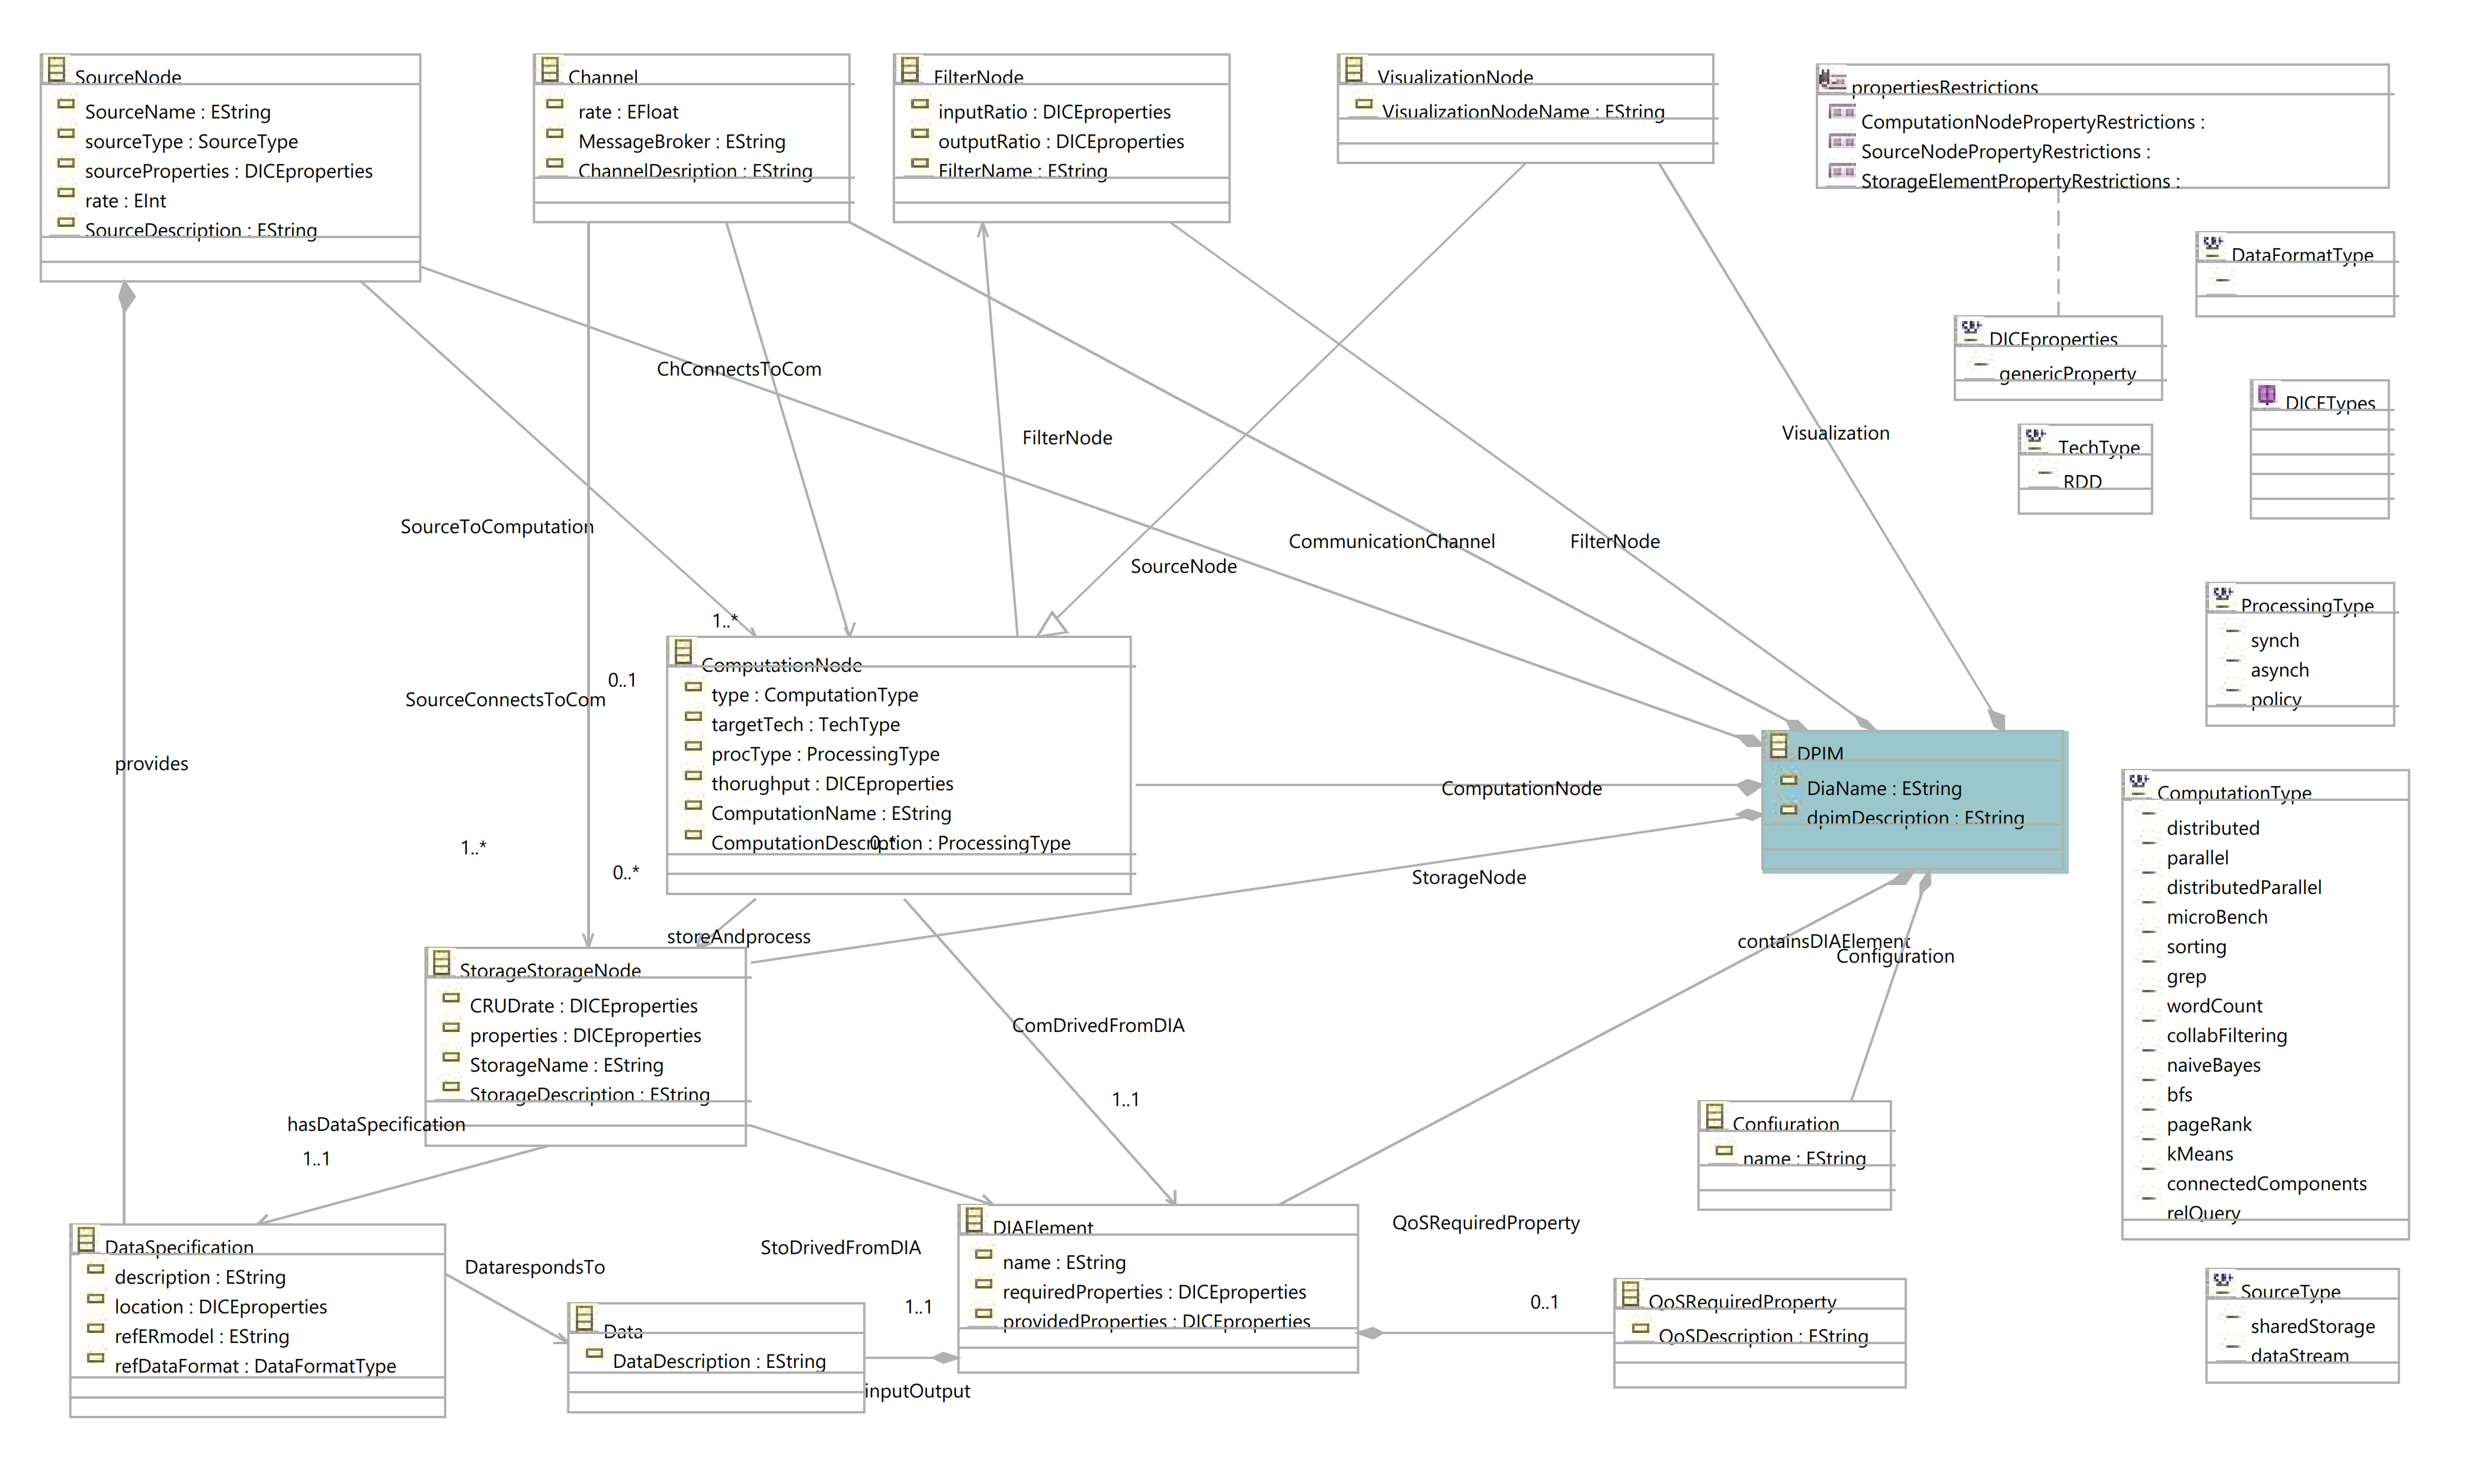
\includegraphics[width=\textwidth]{Images/11.png}
\caption{\label{fig:metamodel}DICE DPIM metamodel.}
\end{sidewaysfigure}


\begin{figure}[H]
	\centering
    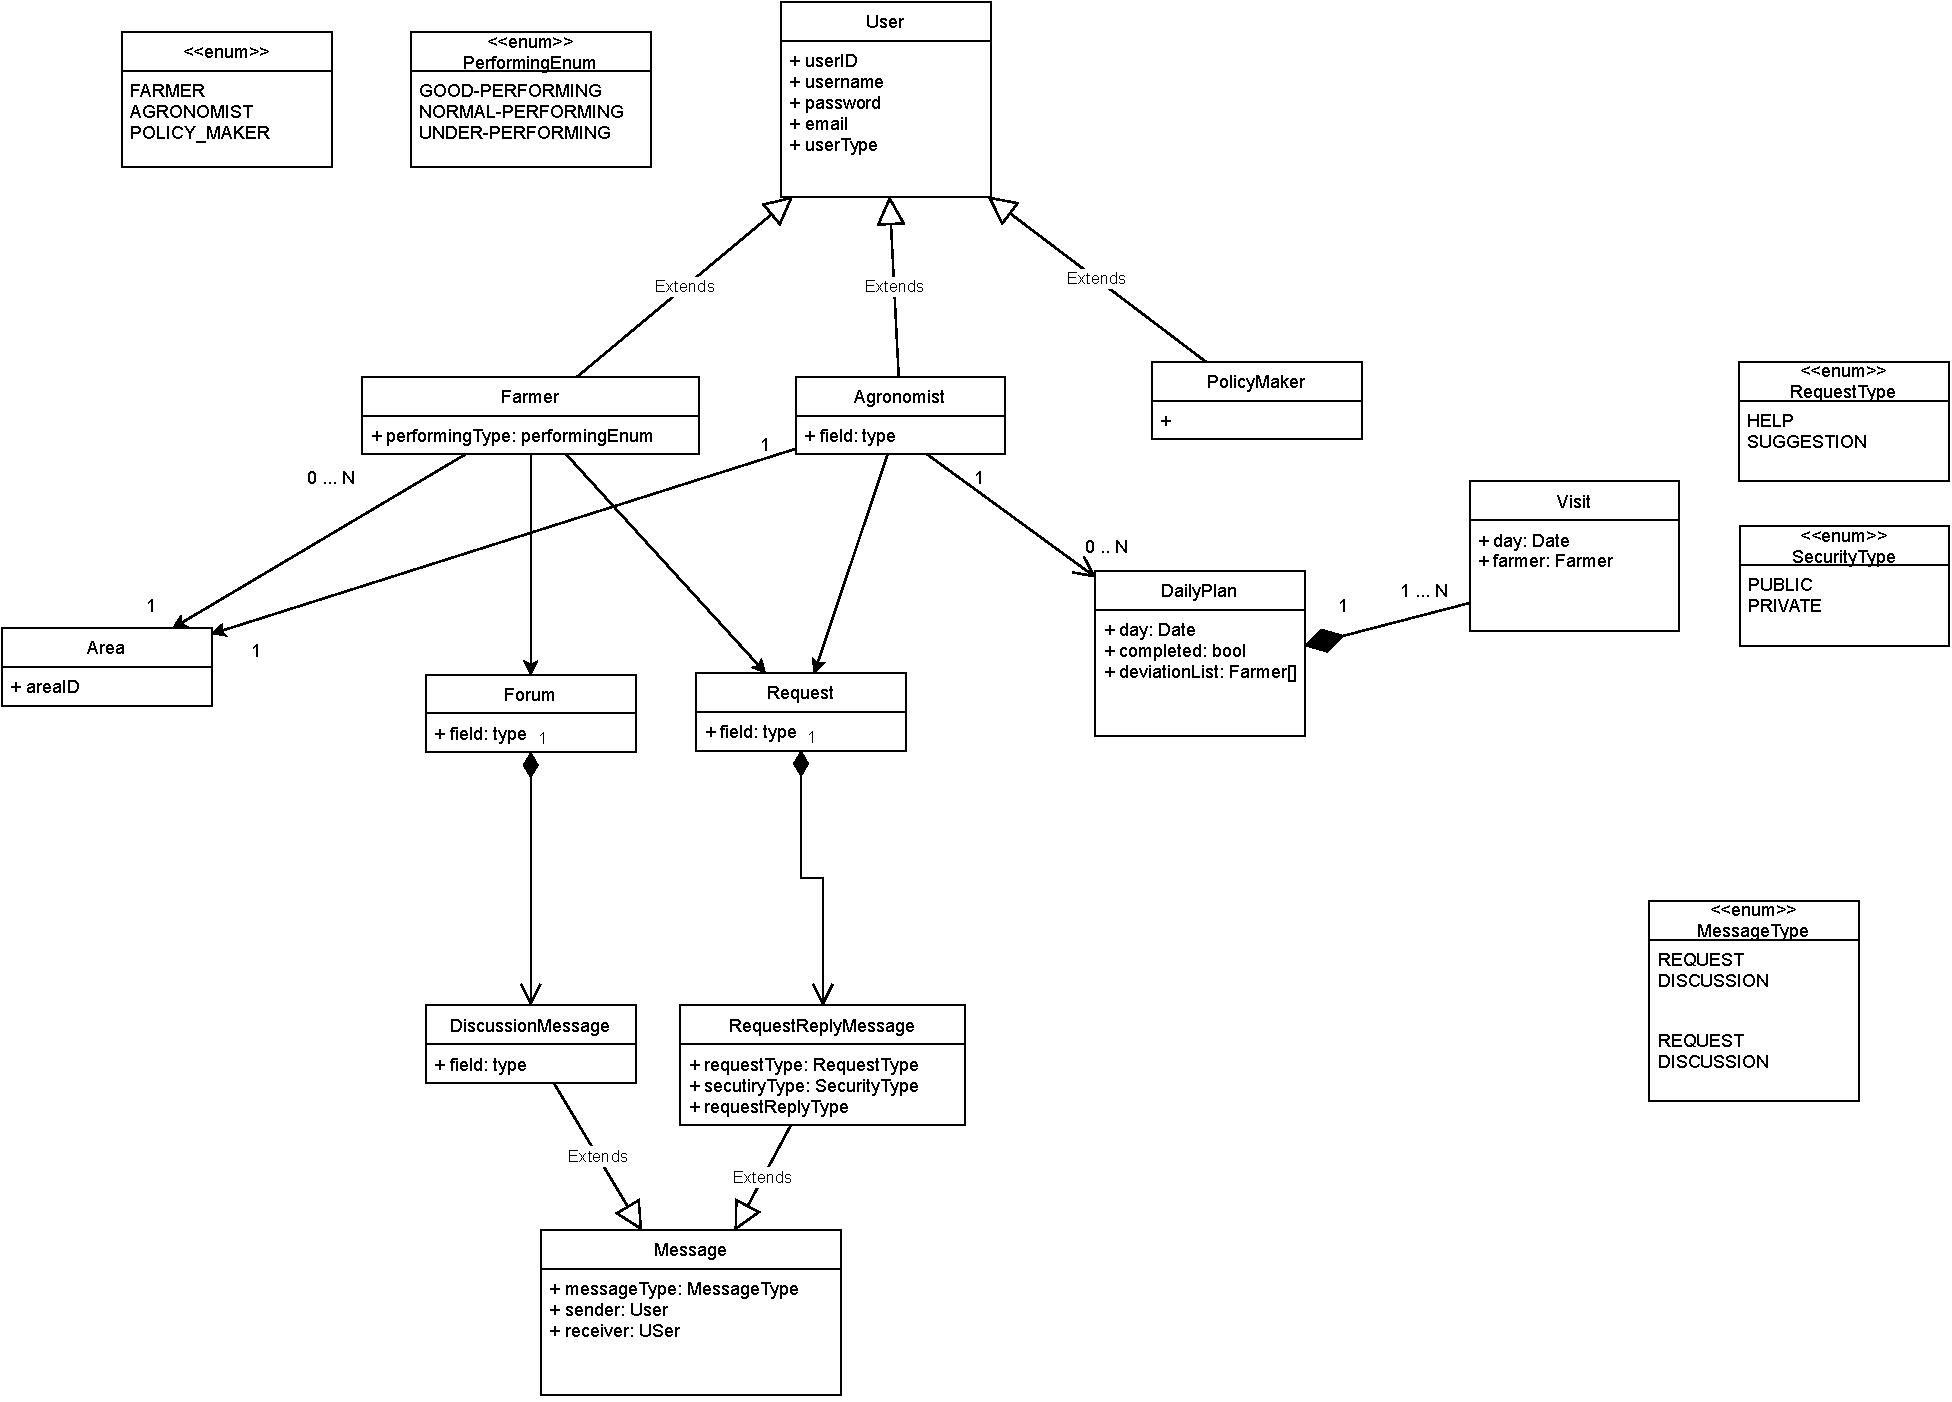
\includegraphics[page=1, width=\textwidth]{Images/SE2 - class diagram.pdf}
	\caption{\label{tab:class_diagram}High level UML diagram}
\end{figure}

\begin{figure}
\centering
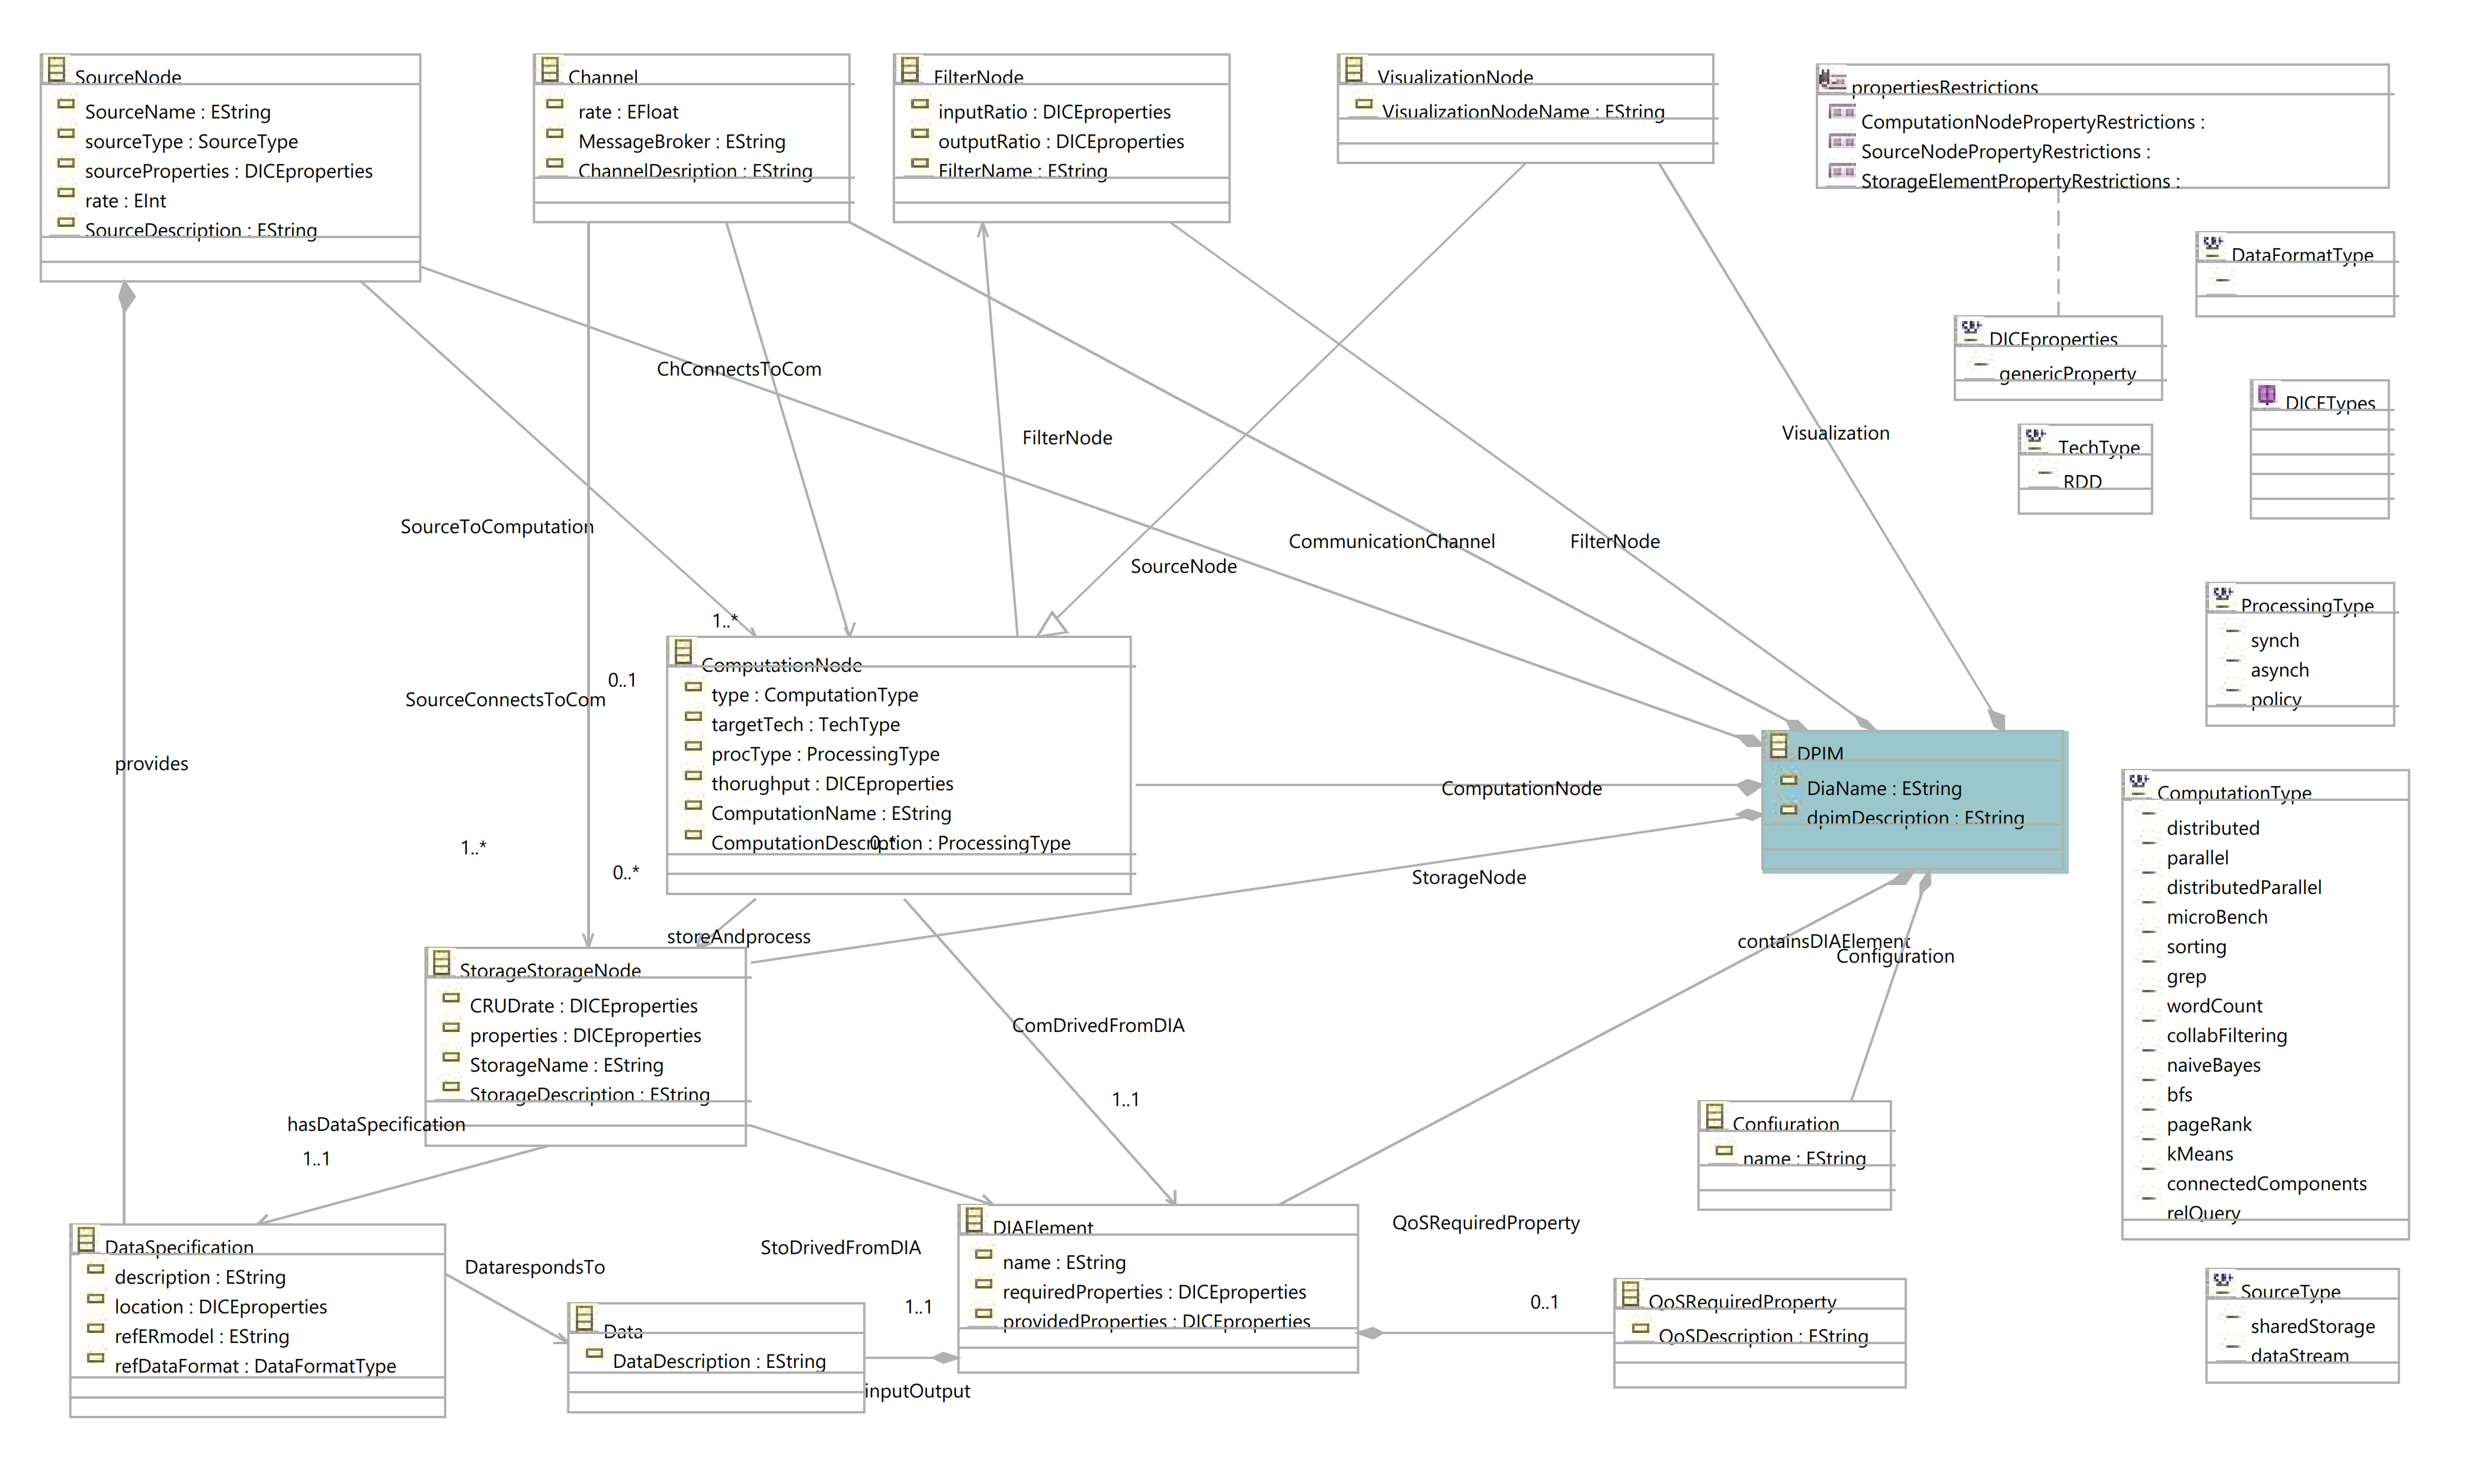
\includegraphics[width=\textwidth]{Images/11.png}
\caption{\label{fig:metamodel2}DICE DPIM metamodel in portrait form.}
\end{figure}

Here is the command to refer to another element (section, figure, table, ...) in the document: \emph{As discussed in Section~\ref{sect:overview} and as shown in Figure~\ref{fig:metamodel}, ...}. Here is how to introduce a bibliographic citation~\cite{DAM}. Bibliographic references should be included in a \texttt{.bib} file. 

Table generation is a bit complicated in Latex. You will soon become proficient, but to start you can rely on tools or external services. See for instance this \href{https://www.tablesgenerator.com}{https://www.tablesgenerator.com}. 
